\chapter{Scenarios and Requirements}
\label{scenario_requirements}
Before attempting to design and implement a secure and restricted ad hoc network, it is important to consider what kind of real life environments they are to be deployed in as they might introduce additional restrictions and requirements on the system. 
\\\\
Emergency situations and military operations are two application areas where ad hoc networks could be very useful as briefly mentioned in Section \ref{ad_hoc_applications}. In this chapter we have focused on describing an example of an emergency response scenario and a typical military scenario where we point out important restrictions and requirements. The chapter continues to describe a simplified and general scenario based on these two which is to be used during our system design and implementation.

\section{Emergency Response Scenario}\label{ems_scen}
Imagine a major natural disaster has hit a densely populated area and the damages to critical communication infrastructure are high. Most of the infrastructure has been destroyed, and what is left rendered useless due to the heavy congestion put upon it. 
\\\\
Right after the disaster has occurred, the local Police force, Paramedics, and Firefighters begin the first phases of the rescue operation. The Police take operational control and they will then need to be able to communicate with the Firefighters and Paramedics to coordinate the operation.
\\\\
Subsequently, different operational centers outside the disaster area are being setup. One center assumes the full operational role and use the local Police as a mediator to the other actors. Some centers take operational role or give assistance to their actors in the field, and some use information from the field to tell the story to the world outside.
\\\\
If need be, some actors such as the Military and private actors such as The Red Cross might also show up. They will also have their own operational centers outside the area, but they are required to submit to the command centers that have the full operational role of the whole disaster area. If no such command centers are already present, they might be the ones taking over that role. Figure \ref{fig:scenario} depicts a full-scale scenario with on-site, as well as off-site actors. The networks in the figure are on different operational planes, shown by the vertical axis.

\begin{figure}[ht!]
  \centering
  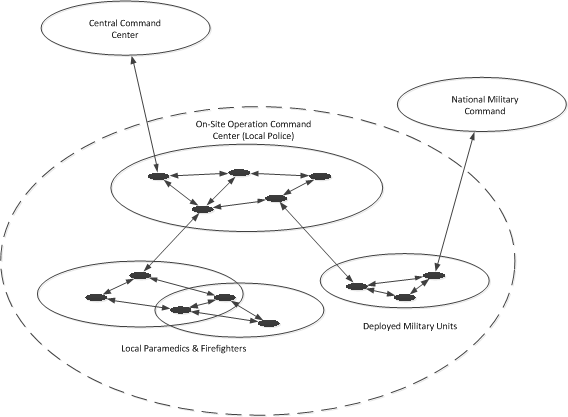
\includegraphics{images/scenario.png}
  \caption{Disaster site with local Police running a Command Center on-site directing the other actors on the site. The figure also shows a military unit getting commands from off-site, as well as the Central Command Center which is in charge of the whole operation from outside.}
  \label{fig:scenario}
\end{figure}


\subsection{Emergency Scenario Requirements} \label{ems_req}
Much of our understanding of the emergency response example scenario is from \cite{ffi_2005_04015}. In an emergency situation there can be many different actors as shown in the example above, e.g. personnel from the Emergency Medical Services, the Fire and Rescue Services, the Police, the Military and private corporations such as the Red Cross.
\\\\
In a typical civilian emergency response there will usually be Fire and Rescue Services, Emergency Medical Services and private actors in the field performing their emergency tasks. The Police will also be in the field managing the whole operation at the site. Outside the field there might be set up different coordinating centers or more professional centers coordinating specific actors in the field.
\\\\
Because emergency responses are usually coordinated efforts between different actors, our system will have to make due with the fact that there might be unknown actors which are not authenticated in the usual sense, for instance if an actor is authenticated by his authority, but that authority is not yet known to the authority in charge of the operational management. If this is the case the actor should maybe have some access to the network resources because they might be very important assets to the operation. This will complicate the authorization process, and we need to determine some set of resources even unauthorized users should have access to.
\\\\
In addition to local access control, we need to control the access to a gateway to the outside world, so that the coordinators outside the field can communicate with the actors in the field.

\section{Military Scenario}\label{mil_scen}
The use of Unmanned Aerial Vehicles (UAV), or drones as they are often referred to in mainstream media, can help foot soldiers in the field by sending them real time video of the site. Foot soldier are thus able to see enemies that are outside of range and visible from the sky. This type of technology can give soldiers huge advantages over their opponents and must be considered very valuable.
\\\\
For this to work, the UAVs need to be able to communicate between each other and with the forces on the ground. They move at a high speed, and do not (usually) operate at the same place twice. This calls for some infrastructure-less communication that can be set up on the fly, quite literally.

\subsection{Military Scenario Requirements} \label{mil_req}
A military setting will typically have higher and stricter requirements regarding the security of the ad hoc network. Here it would be natural to make sure that all nodes and users are properly authorized even to get basic network access. However, there might be some scenarios here too, where getting out information might be more important than authentication, e.g. military orders. That way, even the military might have the requirement of being able to add unknown actors to the network with limited rights.
\\\\  
Secure communication between nodes should be of high importance in military applications. Encrypting messages on the link layer would hide routing information and therefore implicit information of the network topology and nodes from potential adversaries. This may require us to encrypt the whole IP packets or maybe even the wireless link layer frames using 802.11i Robust Security Network (RSN) \cite{citeulike:6535654} or WPA2 \cite{edney2004real}. However, we will not go deeper into link layer encryption, as our main focus is node authentication and not confidentiality.

%\subsection{Scenario Requirements}\label{req_scen}

\section{Our Scenario}
Real life scenarios involving emergency or military operations are complex and many factors affect the situation making it almost impossible to foresee and plan for everything that might happen. The scenarios explained in the sections above presents simple situations showing important operational and organizational aspects that create important requirements that needs to be considered when designing a communications network.
\\\\
Based on the two scenarios described in Section \ref{ems_scen} and \ref{mil_scen}, we define a simpler and more general scenario focusing on the aspects that have the most impact on the communications network while also complementing all the requirements that can be identified from Section \ref{ems_req} and \ref{mil_req}.

\subsection{General Scenario Description}
We imagine that nodes that participate in a communications network belong to different actors that are involved in an emergency or military situation, e.g. the police or the paramedics. To be able to identify themselves to each other they must be in possession of some authentication token, like a certificate, that proves their identity. These tokens might be given according to the different actors to which they belong or they might be issued when a node arrives to a emergency or military scene.
\\\\
In order to have a restricted network there must be some nodes that are in charge of access control to the networks. It is natural to put this responsibility on the entities in the scenarios that already are in charge of operational or administration matters. These master nodes will then be the ones that verify tokens to nodes that wants to enter a restricted network and to issue new tokens to nodes that should be given access to a network. 
\\\\
However, it must also be possible to establish a network without the presence of these master nodes as it might not always be the case that they are in close proximity. Thus other regular nodes must be capable of taking the responsibility for the authentication of nodes in a network.
\\\\
A node should be able to, in some way, join a network even though it does not have a valid token for that network. This is crucial in case the node might have something important to contribute for the e.g. search and rescue operation. However, it might be wise to give this node some limited access and rights in the network since it is not probably authenticated, but enough rights for it to be able to help.
\\\\
Master nodes in different networks should be able to cooperate and merge their networks if this benefits the situation. This entails for some collaboration between these master nodes that gives their nodes access to each others networks.
% some nodes should be able to function as gateways to other network or the internet?

\begin{figure}[ht!]
  \centering
  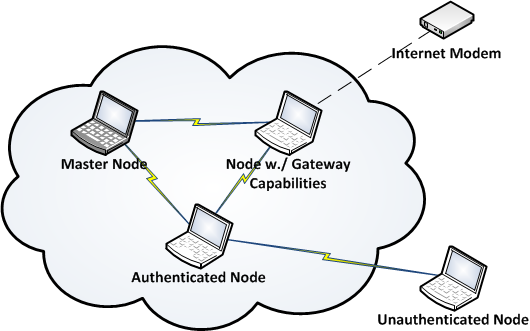
\includegraphics{images/our_scenario.png}
  \caption{Small restricted network with one master node, one authenticated node with gateway capabilities, and one unauthenticated node.}
  \label{fig:our_scenario}
\end{figure}
\noindent
\\\\
In our scenario depicted in Figure \ref{fig:our_scenario} there are three nodes forming the restricted network - one node acting as a master node and one authenticated node with gateway capabilities which makes it possible to communicate with the Internet. Outside the network is an unauthenticated node that needs to be authenticated in some way to join the restricted ad hoc network. It can do so by presenting its authentication certificate to the network, and the master node will verify its identity and decide whether to grant it access or not.

\subsection{Requirements}\label{our_requirements}
Our scenario generates some simple requirements, which we will have to address in our system design. The requirements are summarized in the following table:

\begin{table}[ht!]
	\centering
	\begin{tabular}{ | l | p{11cm} | }
	\hline
	\textbf{Requirement} & \textbf{Requirement Description}\\ \hline
		R1 & A node must be properly authenticated to get full rights in a network  \\ \hline
		R2 & A node which is not properly authenticated should only get limited rights in the network  \\ \hline		
		R3 & A node which is not properly authenticated should be able to full rights after receiving the correct network token \\ \hline
		R4 & All networks should have a master node which handles access control \\ \hline
		R5 & All nodes should be able to assume the role as master node or limited master node \\ \hline
		R6 & Different networks should be able to collaborate \\ \hline
	\end{tabular}
	\caption{Requirements based upon our simplified and general scenario.}
	\label{tab:our_req}
\end{table}

